%auto-ignore
\documentclass[aps,prx,onecolumn,superscriptaddress,floatfix,longbibliography,amsmath,amssymb]{revtex4-2}

\usepackage{xcolor}
\usepackage{graphicx}% Include figure files
\usepackage{hyperref}
\usepackage{dcolumn}% Align table columns on decimal point
\usepackage{bm}% bold math
\usepackage{comment}
\usepackage{dashrule}
\usepackage{accents}

\usepackage{datetime2}
\usepackage{orcidlink}
%%%%

% Equations as (S1), (S2), ...
\renewcommand{\theequation}{S\arabic{equation}}
\setcounter{equation}{0}

\renewcommand{\thesection}{S\arabic{section}}\setcounter{section}{0}
\renewcommand{\thesubsection}{S\arabic{section}.\arabic{subsection}}

\renewcommand{\thefigure}{S\arabic{figure}}
\setcounter{figure}{0}

\renewcommand{\thetable}{S\arabic{table}}
\setcounter{table}{0}

%KTL Added
\newcommand{\ellipse}{\raisebox{-1pt}{\scalebox{1.3}[.4]{$\circ$}}}
\newcommand{\halo}{\accentset{\ellipse}}
\newcommand{\fil}{_{\text F}}
\newcommand{\rfil}{_{\text R}}
\newcommand{\sm}{_{\text S}}
\newcommand{\csm}{_{\rm cS}}
\newcommand{\tar}{_{\rm tar}}
\newcommand{\god}{_{\text T}}
\newcommand{\dd}{{\rm d}}
\newcommand{\bx}{\hat{\bf x}}
\newcommand{\tp}{^\top}
\newcommand{\ex}[1]{\langle #1 \rangle}
\newcommand{\past}[1]{\overleftarrow{#1}}%\overleftarrow{#1}}
\newcommand{\fut}[1]{\overrightarrow{#1}}
\newcommand{\both}[1]{\overleftrightarrow{#1}}
\newcommand{\Tr}{{\rm Tr}}
\newcommand{\inv}{^{-1}}

\newcommand{\beq}{\begin{equation}}
\newcommand{\eeq}{\end{equation}}
\newcommand{\ie}{{\em i.e.}}
\newcommand{\eg}{{\em e.g.}}

\definecolor{nblue}{rgb}{0.06,0.3,0.73}%229 11R, 61G, 145B
\definecolor{nblack}{rgb}{0,0,0}
\definecolor{nred}{rgb}{0.9,0.1,0.1}
\definecolor{nmagenta}{rgb}{0.7,0.0,0.3}
\definecolor{ncyan}{cmyk}{1,0,0,0}
\newcommand{\blu}{\color{nblue}}
\newcommand{\red}{\color{nred}}
\newcommand{\magt}{\color{nmagenta}}
\newcommand{\blk}{\color{nblack}}
\newcommand{\cya}{\color{ncyan}}
\newcommand{\hmw}[1]{\textcolor{red}{\small \bf [[#1]]}}
\newcommand{\ktl}[1]{\textcolor{cyan}{\small \bf [[#1]]}}
\newcommand{\skh}[1]{\textcolor{orange}{\small \bf [[#1]]}}
\newcommand{\rep}[2]{\st{#1}{\red #2}}
\newcommand{\hbx}{\hat\bx}
\newcommand{\hx}{\hat x}

\begin{document}

\title{Supplementary Information for \\ Post-processed estimation of quantum state trajectories}
%\date{\today}

\author{Soroush Khademi}

\author{Jesse J. Slim}

\author{Kiarn T. Laverick}

\author{Jin Chang}

\author{Jingkun Guo}

\author{Simon Gröblacher}

\author{Howard M. Wiseman}

\author{Warwick P. Bowen}

\maketitle

\section{Sample traces of \texorpdfstring{$\langle\hat{X}_1\rangle$}{<X_1>}}\label{sec:DataForX1}

The values of $\langle\hat{X}_1\rangle$, for sample measurement records, are shown in FIG.~\ref{SuppFig:X1&errorbar}\textbf{a} (main experiment) and FIG.~\ref{SuppFig:X1&errorbar}\textbf{c} (noise-injection experiment). They are qualitatively similar to the sample traces of $\langle\hat{X}_2\rangle$ shown in FIG.~\ref{FigData1}\textbf{b} and FIG.~\ref{FigData3}\textbf{b}, as $\hat{X}_1$ and $\hat{X}_2$ have identical statistics due to dynamical symmetry. 

\section{Extended data for $\delta_\text{C}$}

The distributions of $\delta_\text{C}(t)=\langle\hat{X}_j\rangle_\text{F}^\text{LTL}(t)-\langle\hat{X}_j\rangle_\text{C}(t),\;j=1,2$ for three sample times are shown in FIG.~\ref{SuppFig:delta_C}. They all have zero means. That is, filtering (C = F) and quantum state smoothing (C = S) are unbiased estimations of the target mean values. Interestingly, the classical smoothing (C = cS) distributions are also unbiased. The standard deviations of all distributions decrease over time, as also shown by FIG.~\ref{FigData1}\textbf{c}, with the quantum state smoothing ones remaining the smallest.

\section{Inference self-consistency relations}\label{SecConsistency}

In this section, we examine the equality $\mathbb{V}\text{ar}_{\text{ens}}\big[\langle\hat{X}_j\rangle_\text{C}(t)\big]=\sigma^2_\text{uncon}-v_\text{C}(t)$ for an infinitely large ensemble of measurement records. The effect of the finite size of the experimental ensemble is discussed in the next section.

For filtering ($\text{C}=\text{F}$), Eq.~\eqref{equ:rFT} gives
\beq
\ex{\hat{X}_j}\fil(t) = e^{-\Gamma t/2}\ex{\hat{X}_j}\fil(0) + \sqrt{2\eta\Gamma {\cal C}}\int_{0}^{t} e^{-\frac{\Gamma}{2}(t - s)} v\fil(s)\dd W_{{\rm F},j}(s)\,.
\eeq
Considering $\mathbb{V}\text{ar}_{\text{ens}}\big[\langle\hat{X}_j\rangle_\text{F}(t)\big]={\mathbb E}_{\text{ens}}\big[\ex{\hat{X}_j}_\text{F}^2(t)\big] - {\mathbb E}^2_{\text{ens}}\big[\ex{\hat{X}_j}\fil(t)\big]$, where ${\mathbb E}_{\text{ens}}[\bullet]$ denotes averaging, ${\mathbb E}_{\text{ens}}\big[\dd W_{{\rm F},j}(s)\big] = 0$ and ${\mathbb E}_{\text{ens}}\big[\dd W_{{\rm F},j}(s)\,\dd W_{{\rm F},j}(s')\big] = \delta(s-s')\,\dd s^2$, we find
\beq
\mathbb{V}\text{ar}_{\text{ens}}\big[\langle\hat{X}_j\rangle_\text{F}(t)\big] = e^{-\Gamma t}\,\mathbb{V}\text{ar}_{\text{ens}}\big[\langle\hat{X}_j\rangle_\text{F}(0)\big] + 2\eta\Gamma \mathcal{C}\int_{0}^{t} \dd s\,e^{-\Gamma (t - s)}v^2_\text{F}(s)\,. 
\eeq
%In order to validate the theoretical models of our system, we compute the ensemble variance of the filtered means, $v\fil^{\rm ens}(t) = {\mathbb E}\{\ex{\hat{X}_j}\fil(t)^2\} - {\mathbb E}\{\ex{\hat{X}_j}\fil(t)\}^2$, where ${\mathbb E}\{\bullet\}$ denotes an ensemble average. To compare this experimentally accessible variance to the theory, we begin my solving the stochastic differential equation for the filtered mean Eq.~(\ref{equ:rFT}). It is easy to show that the filtered mean at any time is given by
%\beq
%\ex{\hat{X}_j}\fil(t) = e^{-\frac{\Gamma}{2} (t - t_0)}\ex{\hat{X}_j}\fil(t_0) + \sqrt{2\eta\Gamma {\cal C}}\int_{t_0}^{t} e^{-\frac{\Gamma}{2}(t - s)} v\fil(s)\dd W_{{\rm F},j}(s)\,.
%\eeq
%Since, in the limit where the number of ensembles sampled goes to infinity, we expect the ensemble average to equal the theoretical statistical average, as well as a very good approximation for a large but finite number of samples. Thus, we can expect that ${\mathbb E}\{\dd W_{{\rm F},j}(s)\} = 0$ and ${\mathbb E}\{\dd W_{{\rm F},j}(s)\dd W_{{\rm F},j}(s')\} = \delta(s - s')\dd s$. Computing the ensemble variance gives
%\beq
%v\fil^{\rm ens}(t) = e^{-\Gamma (t - t_0)}v\fil^{\rm ens}(t_0) + 2\eta\Gamma \mathcal{C}\int_{t_0}^{t} \dd s e^{-\Gamma (t - s)}v\fil(s)^2\,. 
%\eeq
%Note, since $\ex{\hat X_j}\fil(t_0)$ is fixed by the initial condition, $v\fil^{\rm ens}(t_0) = 0$. Thus, we have 
%\beq
%v\fil^{\rm ens}(t) = 2\eta\Gamma \mathcal{C}\int_{t_0}^{t} \dd s e^{-\Gamma (t - s)}v\fil(s)^2\,. 
%\eeq
As $\ex{\hat X_j}\fil(0)$ is fixed (at zero), $\mathbb{V}\text{ar}_{\text{ens}}\big[\langle\hat{X}_j\rangle_\text{F}(0)\big] = 0$ and 
\beq
\mathbb{V}\text{ar}_{\text{ens}}\big[\langle\hat{X}_j\rangle_\text{F}(t)\big] = 2\eta\Gamma \mathcal{C}\int_{0}^{t} \dd s\,e^{-\Gamma (t - s)}v^2_\text{F}(s)\,.
\label{eq:intv2}
\eeq
Let us now also consider the quantity $\ell(t) = \sigma^2_\text{uncon} - v\fil(t)$. Considering Eq.~(\ref{NLODE}), we have
\beq
\frac{\dd}{\dd t}\ell(t) = -\Gamma \ell(t) + 2\eta\Gamma \mathcal{C} v^2_\text{F}(t)\,,
\eeq
which has the solution
\beq
\ell(t) = e^{-\Gamma t}\ell(0) + 2\eta\Gamma \mathcal{C} \int_{0}^{t}\dd s\,e^{-\Gamma (t - s)}v^2_\text{F}(s)\,.
\eeq
As $v\fil(0) = \sigma^2_\text{uncon}$, $\ell(0) = 0$ and 
\beq
\ell(t) = 2\eta\Gamma \mathcal{C} \int_{0}^{t}\dd s\,e^{-\Gamma (t - s)}v^2_\text{F}(s)\,.
\label{eq:lt}
\eeq
We can therefore conclude from Eqs.~\eqref{eq:intv2} and \eqref{eq:lt} that
\beq
\mathbb{V}\text{ar}_{\text{ens}}\big[\langle\hat{X}_j\rangle_\text{F}(t)\big] = \ell(t) = \sigma^2_\text{uncon} - v\fil(t)\,.
\label{equ:Inf_Consistency_F}
\eeq

\begin{figure*}[t!]
    \centering
    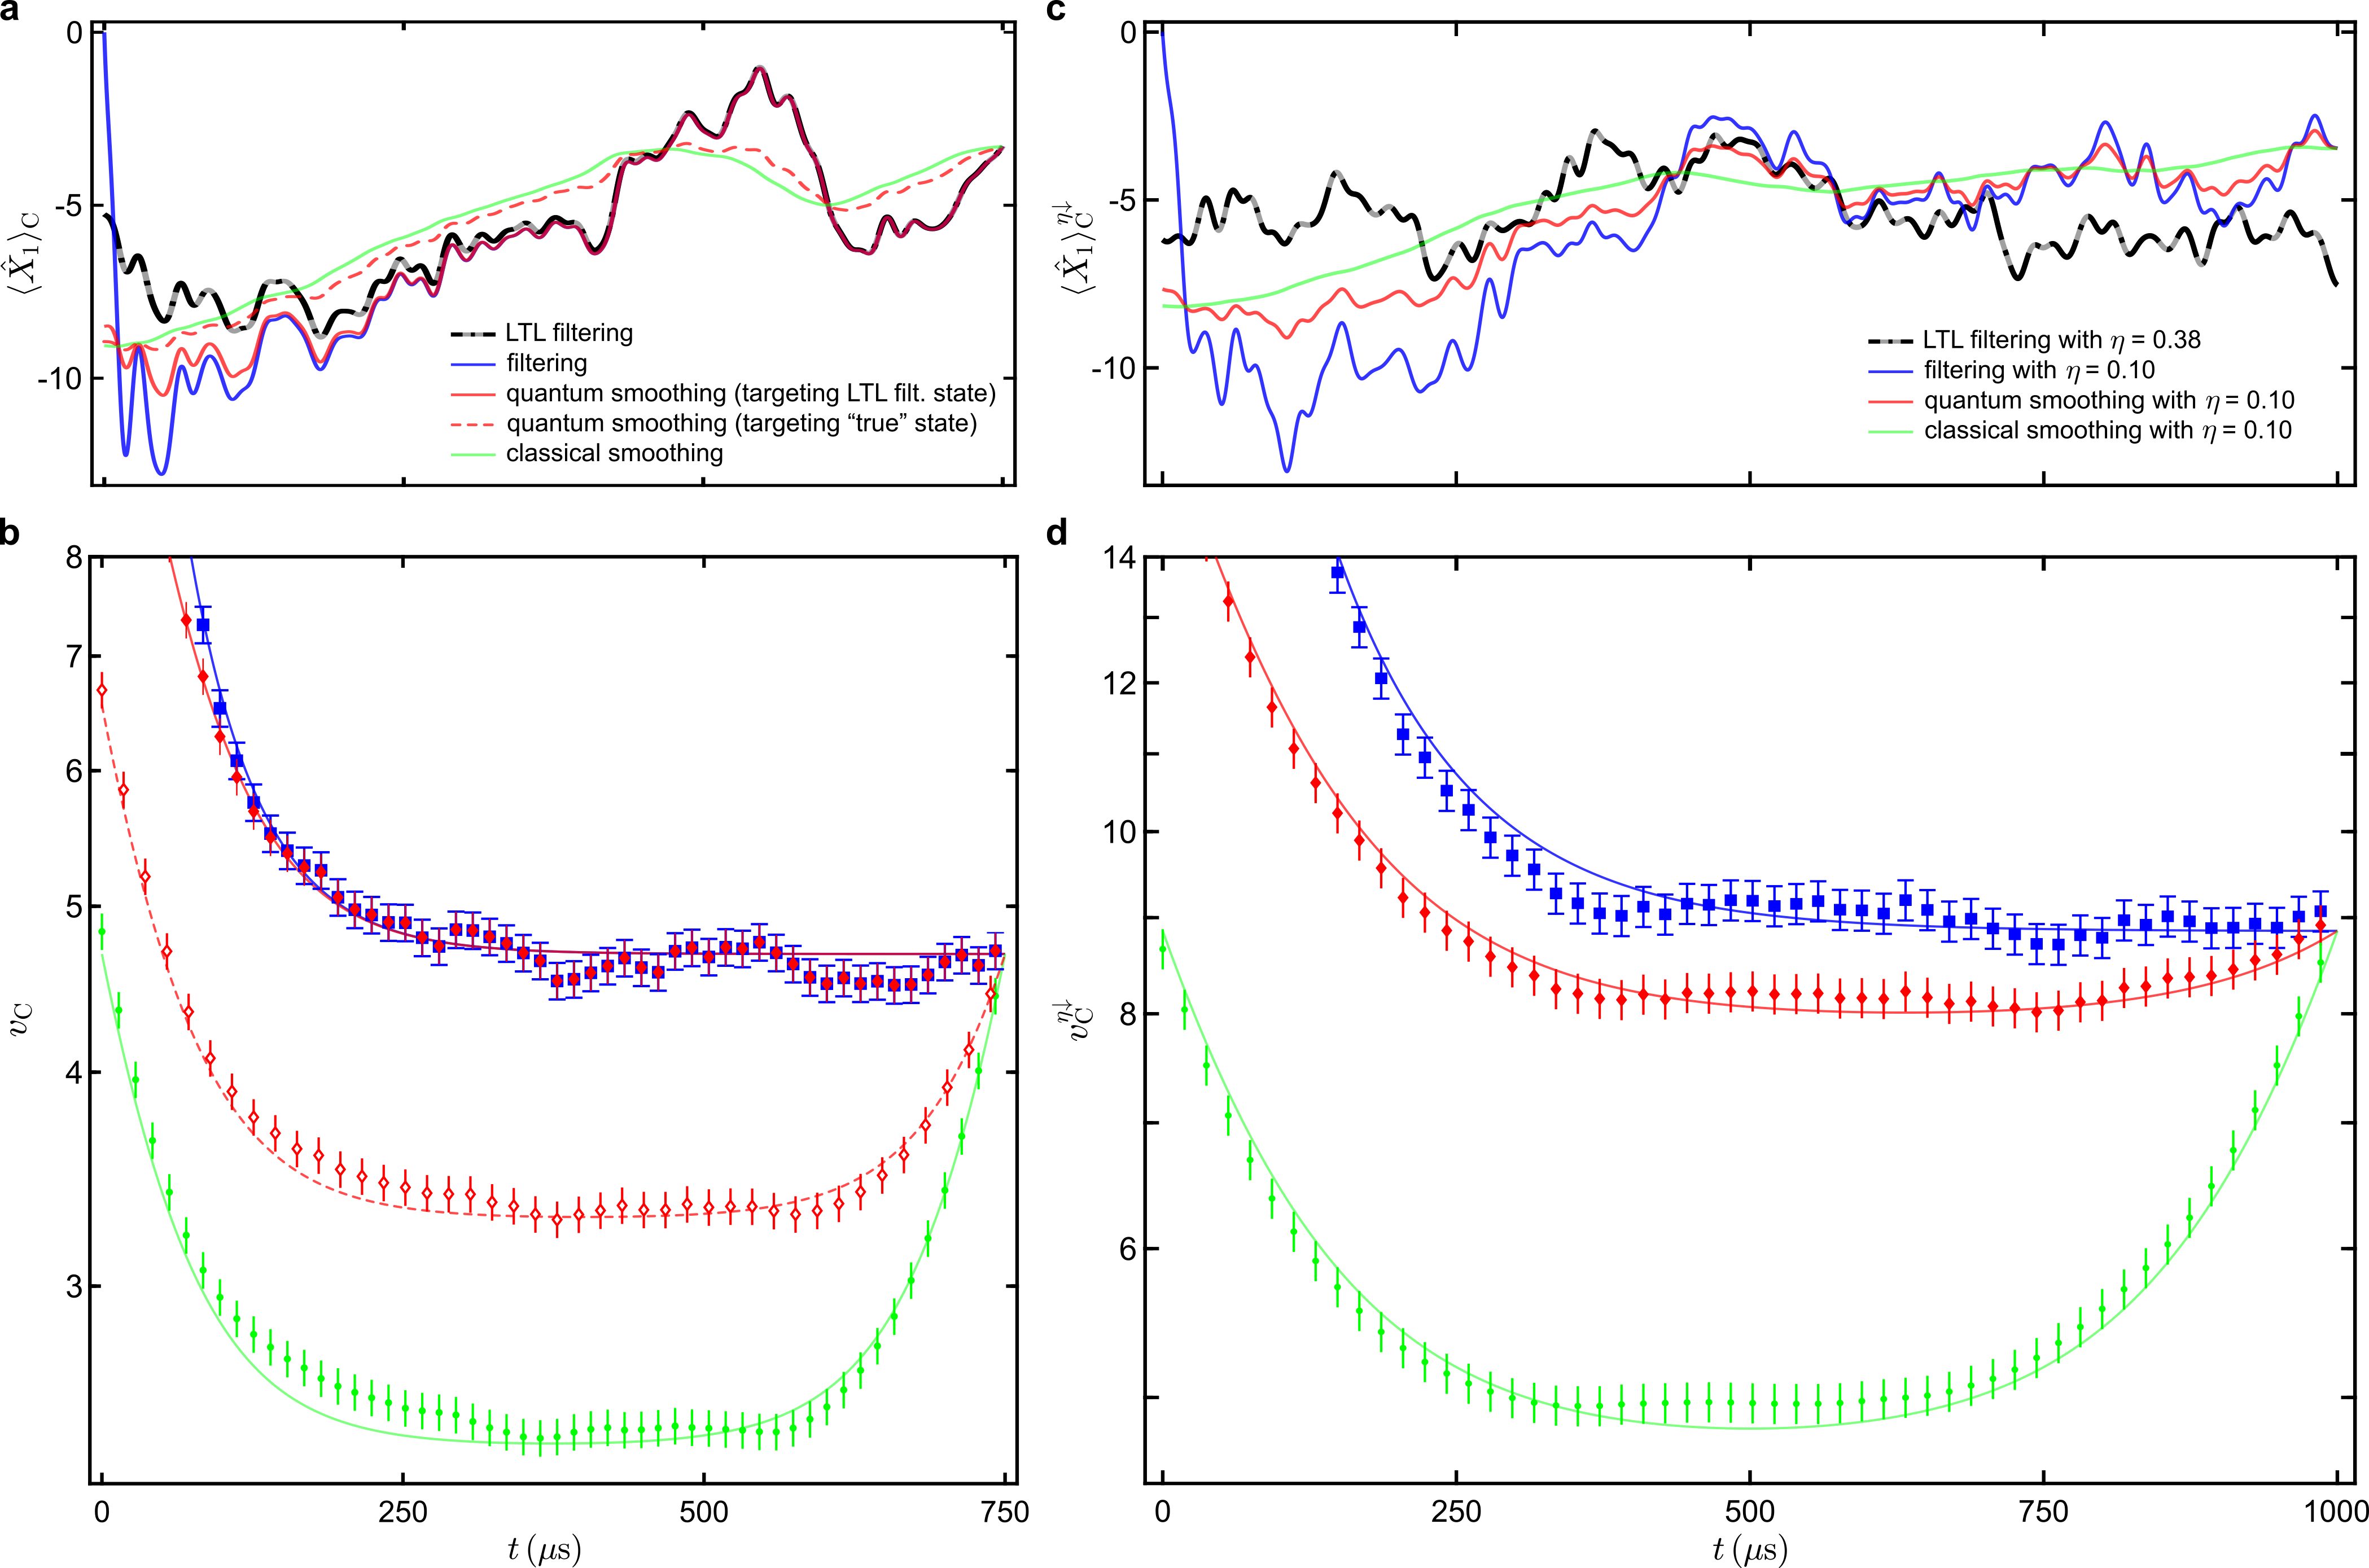
\includegraphics[]{matSupp_figs/FigSupp2.png}
    \caption{\textbf{Estimation analysis extended data.} \textbf{a-b,} The main experiment data.
    %: filtering (blue), quantum smoothing with the LTL filtered state target (solid red), quantum smoothing with the ``true" state target (dashed red) and classical smoothing (green)
    \textbf{a,} Stochastic traces for the quadrate mean $\langle\hat{X}_1\rangle(t)$ for a sample measurement record. \textbf{b,} Deterministic conditional variances ($v_\text{C}(t)$, curves) and the corresponding value of $\sigma^2_\text{uncon}-\mathbb{V}\mathrm{ar}_{\text{ens}}[\langle\hat{X}_j\rangle_\text{C}(t)]$ (data points) with error bars. \textbf{c-d,} The noise-injection ($\eta$-reduced) experiment data.
    %: filtering (blue), quantum smoothing with the initial-$\eta$ LTL filtered state target (solid red) and classical smoothing (green)
    \textbf{c,} Stochastic traces for the quadrate mean $\langle\hat{X}_1\rangle(t)$ for a sample measurement record. \textbf{d,} Deterministic conditional variances ($v_\text{C}^{\eta\downarrow}(t)$, curves) and the corresponding value of $\sigma^2_\text{uncon}-\mathbb{V}\mathrm{ar}_{\text{ens}}[\langle\hat{X}_j\rangle_\text{C}^{\eta\downarrow}(t)]$ (data points) with error bars. In \textbf{b} and \textbf{d}, the vertical axes are limited to near steady-state values for visual clarity, and each error bar spans two standard deviations of the error (caused by the finite size of the ensemble of measurement records).}
    \label{SuppFig:X1&errorbar}
\end{figure*}

To examine the case of quantum state smoothing ($\text{C}=\text{S}$), we note that
\begin{equation}
\begin{array}{rcl}
    \mathbb{V}\text{ar}_{\text{ens}}\big[\langle\hat{X}_j\rangle_\text{S}(t)\big] & = & \left(\dfrac{v\sm-v\tar}{v\fil-v\tar}\right)^2\;\mathbb{V}\text{ar}_{\text{ens}}\big[\langle\hat{X}_j\rangle_\text{F}(t)\big]+\\&&\left(\dfrac{v\sm-v\tar}{v\rfil+v\tar}\right)^2\;\mathbb{V}\text{ar}_{\text{ens}}\big[\langle\hat{X}_j\rangle_\text{R}(t)\big]+\\&&
    2\left(\dfrac{v\sm-v\tar}{v\fil-v\tar}\right)\left(\dfrac{v\sm-v\tar}{v\rfil+v\tar}\right)\;
    \mathbb{C}\text{ov}_{\text{ens}}\big[\langle\hat{X}_j\rangle_\text{F}(t),\langle\hat{X}_j\rangle_\text{R}(t)\big]
    \label{equ:VarX_S}
\end{array}
\end{equation}
where $v\tar$ is the variance of the target state. To evaluate this expression, we first investigate the value of $\mathbb{V}\text{ar}_{\text{ens}}\big[\langle\hat{X}_j\rangle_\text{R}(t)\big]$.
%, where the mean is given by (Eqs.~\eqref{1stmomentNREO} and~\eqref{IPmatrices})
%\begin{equation}
%    -\dd\langle \hat{X}_j \rangle_R(t) = \dfrac{\Gamma}{2}\,\langle\hat{X}_j \rangle_R(t)\,\dd t+\sqrt{2\eta\Gamma \mathcal{C}}\,v_R(t)\,\dd W_{R,j}(t)\,,\;\;\;\text{j}=1,2
%\end{equation}
%where
%\begin{equation}
%    \dd W_{\text{R},j}(t) =\text{I}_{j}(t)\,\dd t - \sqrt{2\eta\Gamma \mathcal{C}}\;\dd t\;\langle\hat{X}_\text{j} \rangle_R(t)\,.
%\end{equation}
%{\cya In order to determine $\mathbb{V}\text{ar}_{\text{ens}}\big[\langle\hat{X}_j\rangle_\text{R}(t)\big]$,
Considering the definition of the retrofiltered effect operator, we have $p(\fut{O}_t|\rho_{\rm uncon}) \propto \Tr[\hat E\rfil\rho_{\rm uncon}]$. Given that both the effect operator and the unconditional state are Gaussian, and that $\Tr[\rho\sigma] = 4\pi\int\dd{\bf x} W_{\rho}({\bf x})W_{\sigma}({\bf x})$, we find 
\beq
p(\fut{O}_t|\rho_{\rm uncon}) \propto g(\ex{\bx}\rfil;\ex{\bx}_{\rm uncon}, {\rm V}\rfil + {\bf V}_{\rm unc})\equiv p(\ex{\bx}\rfil;t)
\eeq
where the final equivalence comes from the fact that $\ex{\bx}\rfil(t)$ is a deterministic function of $\fut{O}_t$, with the other variables in the Gaussian being independent of the measurement records.
%Now that we have the distribution for $\ex{\bx}\rfil(t)$, we can analytically compute the variance for our system via
The standard probability theory then yields
\beq\label{equ:Inf_Consistency_R}
\mathbb{V}\text{ar}_{\rm ens}\big[\langle\hat{X}_j\rangle_\text{R}(t)\big] = \sigma_{\rm uncon}^2 + v\rfil(t)\,.
\eeq
\begin{figure*}[t!]
    \centering
    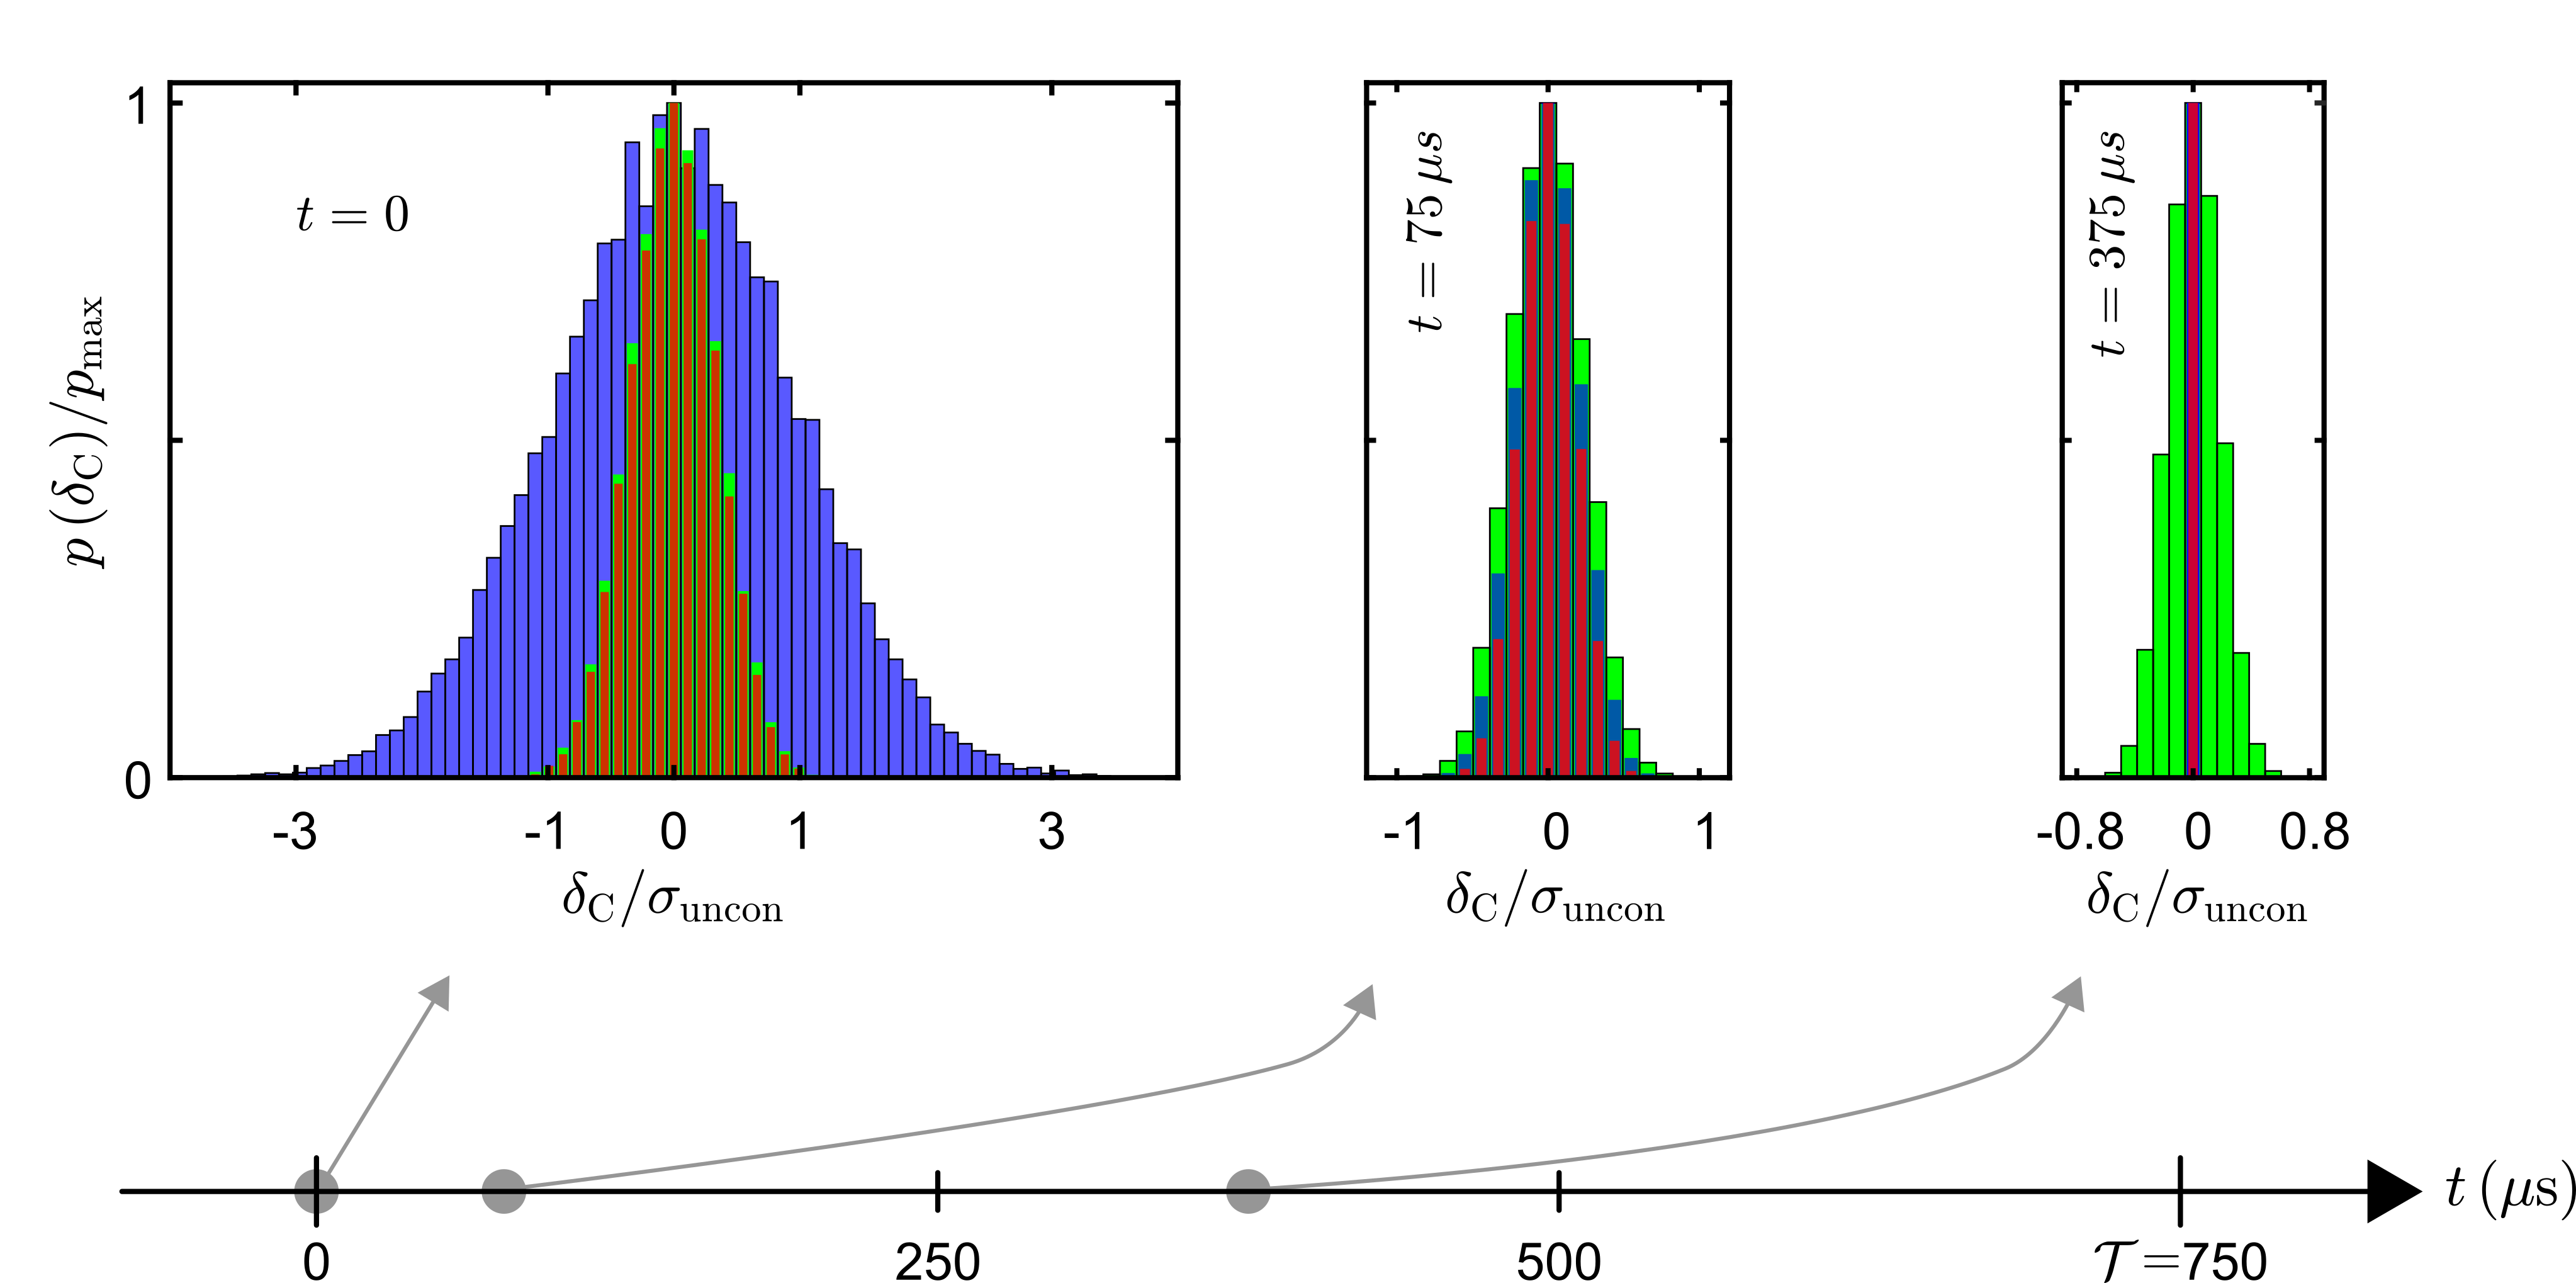
\includegraphics[]{matSupp_figs/FigSupp1.png}
    \caption{\textbf{Distributions of} $\delta_\text{C}(t)=\langle\hat{X}_j\rangle_\text{F}^\text{LTL}(t)-\langle\hat{X}_j\rangle_\text{C}(t),\;j=1,2$\textbf{.} With the main experiment data, the blue histograms are for C = F (filtering), the red ones for C = S (quantum smoothing) and the green ones for C = cS (classical smoothing). $p(\delta_\text{C})$ is the probability distribution of the realised $\delta_\text{C}$ values and $p_\text{max}$ is the maximum bar height of the corresponding histogram.}
    \label{SuppFig:delta_C}
\end{figure*}
%Similarly, to verify the retrofiltered variance, we similarly consider $v\rfil^{\rm ens}(t) = {\mathbb E}\{\ex{\hat{X}_j}\rfil(t)^2\} - {\mathbb E}\{\ex{\hat{X}_j}\rfil(t)\}^2$. Solving (formally) for the retrofiltered mean, one finds
%{\color{orange} Kiarn, Could you please polish your retro-filtering derivation? I commented out mine. Thanks man for putting time during your holidays.
%I should sit with you after the submission to better understand the mathematics of the complication existing around the direction of the differential equations --- I do not see any difference between
%\begin{equation}
%    \begin{array}{rl}
%     -dx= &\Gamma/2\;x\,dt\rightarrow x(t-dt)-x(t)=\Gamma/2\;x(t)\,dt\rightarrow \\ x(t-dt)= & (1+\Gamma/2\;dt)\,x(t)=\exp(\Gamma/2\;dt)\,x(t)\rightarrow x(t)=\exp(-\Gamma/2\;dt)\,x(t-dt)
%    \end{array}
%\end{equation}
%and
%\begin{equation}
%    \begin{array}{rl}
%     -dx= &\Gamma/2\;x\,dt\rightarrow dx= -\Gamma/2\;x\,dt\rightarrow x(t+dt)-x(t)=-\Gamma/2\;x(t)\,dt\rightarrow \\ x(t+dt)= & (1-\Gamma/2\;dt)\,x(t)=\exp(-\Gamma/2\;dt)\,x(t)\;.
%    \end{array}
%\end{equation}
%This is not for you to reply, just saying why I still do not understand and need to talk about it in the future -- even the blow-up argument doesn't satisfy me as $\ex{\hat{X}_j}\rfil(\mathcal{T})$ is undefined.} \ktl{I agree for the mean the blow-up argument is not true, but when you get to the variance, that is when the argument holds}\skh{Anyway, your current derivation makes sense to me and is very nice and short.}
\begin{comment}
By solving this equation, we find
\beq
\ex{\hat{X}_j}\rfil(t) = e^{-\Gamma t/2}\,\ex{\hat{X}_j}\rfil(0) - \sqrt{2\eta\Gamma \mathcal{C}}\int_{0}^{t}e^{-\frac{\Gamma}{2}(t-s)}v\rfil(s)\,\dd W_{{\rm R},j}(s)\,.
\eeq
Considering $\mathbb{V}\text{ar}_{\text{ens}}\big[\langle\hat{X}_j\rangle_\text{R}(t)\big]={\mathbb E}_{\text{ens}}\big[\ex{\hat{X}_j}\rfil^2(t)\big] - {\mathbb E}^2_{\text{ens}}\big[\ex{\hat{X}_j}\rfil(t)\big]$, ${\mathbb E}_{\text{ens}}\big[\dd W_{{\rm R},j}(s)\,\dd W_{{\rm R},j}(s')\big] = \delta(s-s')\,\dd s^2$ and ${\mathbb E}_{\text{ens}}\big[\dd W_{{\rm R},j}(s)\big] = 0$, we have
\begin{equation}
\begin{array}{rcl}
\mathbb{V}\text{ar}_{\text{ens}}\big[\langle\hat{X}_j\rangle_\text{R}(t)\big] & = & e^{-\Gamma t}\,\mathbb{V}\text{ar}_{\text{ens}}\big[\langle\hat{X}_j\rangle_\text{R}(0)\big] + 2\eta\Gamma \mathcal{C}\displaystyle\int_{0}^{t}\dd s e^{-\Gamma(t-s)}v^2_\text{R}(s) \\ && \\ && - 2\sqrt{2\eta\Gamma \mathcal{C}}\displaystyle\int_{0}^{t}e^{-\frac{\Gamma}{2}(t-s)}v\rfil(s)\,{\mathbb E}_{\text{ens}}\big[\ex{\hat{X}_j}\rfil(0)\,\dd W_{{\rm R},j}(s)\big]
\end{array}
\end{equation}
\begin{figure*}[t!]
    \centering
    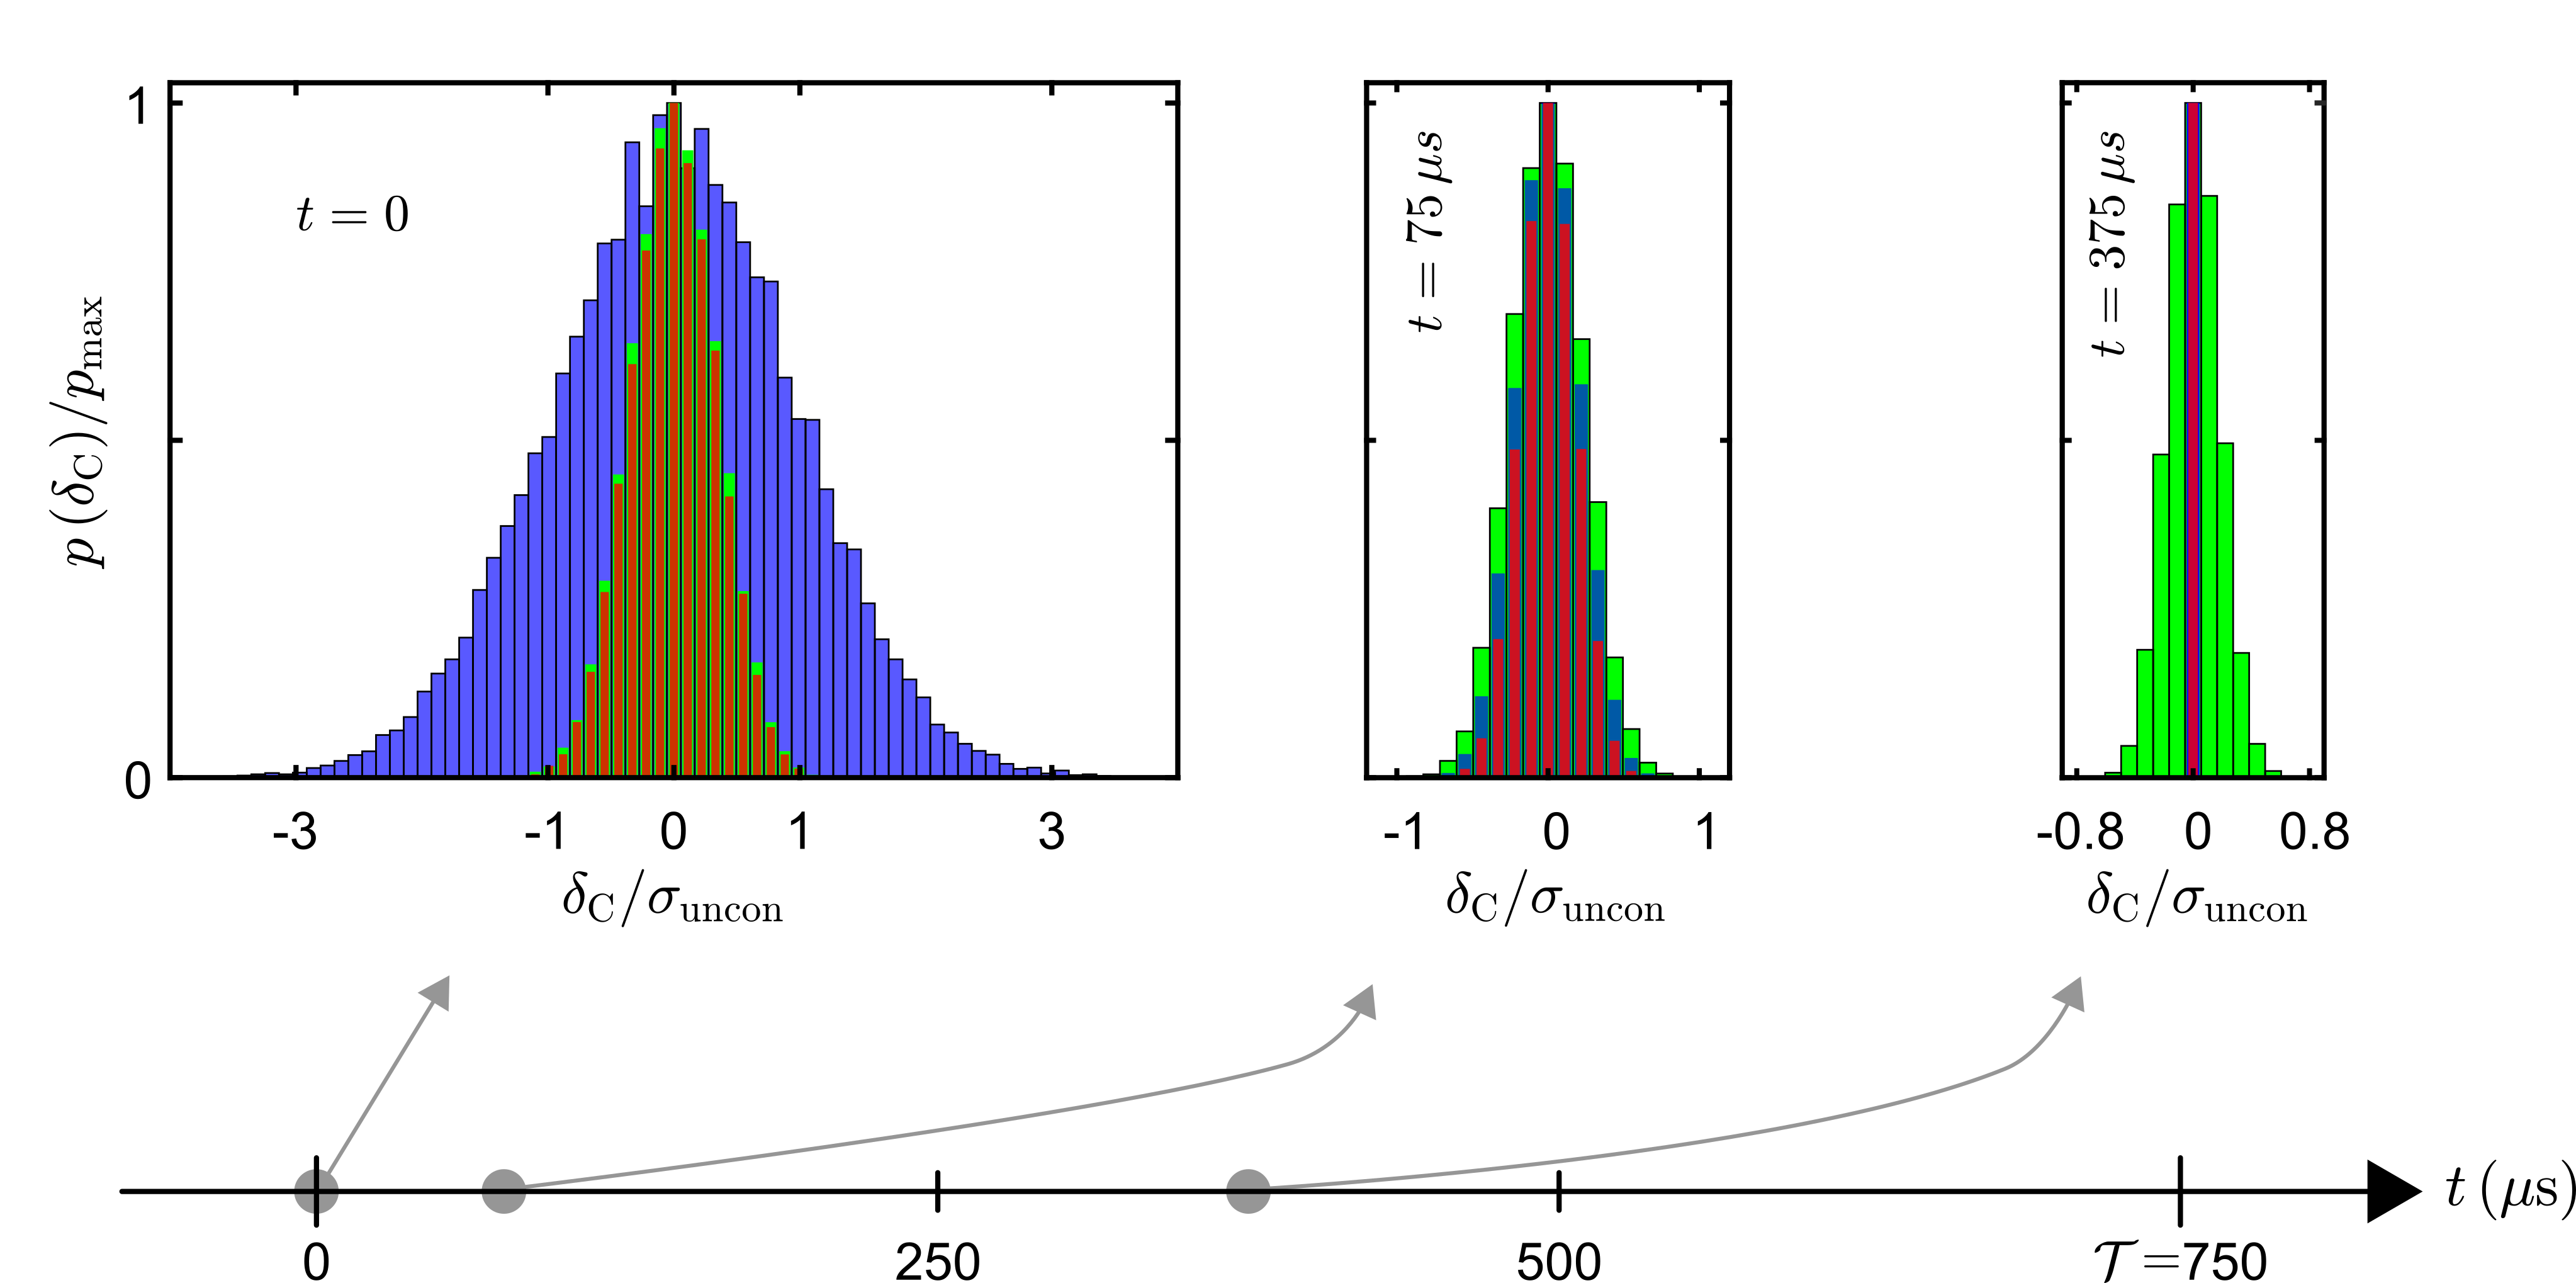
\includegraphics[]{matSupp_figs/FigSupp1.png}
    \caption{\textbf{Distributions of} $\delta_\text{C}(t)=\langle\hat{X}_j\rangle_\text{F}^\text{LTL}(t)-\langle\hat{X}_j\rangle_\text{C}(t),\;j=1,2$\textbf{.} With the main experiment data, the blue histograms are for C = F (filtering), the red ones for C = S (quantum smoothing) and the green ones for C = cS (classical smoothing). $p(\delta_\text{C})$ is the probability distribution of the realised $\delta_\text{C}$ values and $p_\text{max}$ is the maximum bar height of the corresponding histogram.}
    \label{SuppFig:delta_C}
\end{figure*}
where ${\mathbb E}_{\text{ens}}\big[\ex{\hat{X}_j}\rfil(0)\,\dd W_{{\rm R},j}(s)\big]\propto{\mathbb E}_{\text{ens}}\big[\big(\text{I}_j(0)\dd t-\dd W_{{\rm R},j}(0)\big)\,\dd W_{{\rm R},j}(s)\big]$, which is, in turn, proportional to $\delta(s)\dd s^2$ as $\text{I}_j(0)$ in independent of the value of $\mathcal{T}$. Therefore, the last term on the right hand side disappears and 
\begin{equation}
\begin{array}{rcl}
\mathbb{V}\text{ar}_{\text{ens}}\big[\langle\hat{X}_j\rangle_\text{R}(t)\big] & = & e^{-\Gamma t}\,\mathbb{V}\text{ar}_{\text{ens}}\big[\langle\hat{X}_j\rangle_\text{R}(0)\big] + 2\eta\Gamma \mathcal{C}\displaystyle\int_{0}^{t}\dd s e^{-\Gamma(t-s)}v^2_\text{R}(s)
\label{equ:MyV}
\end{array}
\end{equation}
Let us now consider $k(t) = \sigma^2_\text{uncon} + v\rfil(t)$. Considering Eqs.~(\ref{2ndmomentNREO}) and (\ref{IPmatrices}), we get
\beq
\frac{\dd}{\dd t}k(t) = -\Gamma k(t) + 2\eta\Gamma \mathcal{C} v^2_\text{R}(t)\,,
\eeq
which has the solution
\beq
k(t) = e^{-\Gamma t}k(0) + 2\eta\Gamma \mathcal{C} \int_{0}^{t}\dd s e^{-\Gamma (t-s)}v^2_\text{R}(s)
\label{equ:Myk}
\eeq
Considering Eqs.~\eqref{equ:MyV} and~\eqref{equ:Myk}, we have
\begin{equation}
    \mathbb{V}\text{ar}_{\text{ens}}\big[\langle\hat{X}_j\rangle_\text{R}(t)\big] -k(t) = e^{-\Gamma t}\times\left(\mathbb{V}\text{ar}_{\text{ens}}\big[\langle\hat{X}_j\rangle_\text{R}(0)\big]-k(0)\right)
\label{equ:MyV-k}
\end{equation}
In case the two sides of this equation were none-zero, we could write
\begin{equation}
    \dfrac{\mathbb{V}\text{ar}_{\text{ens}}\big[\langle\hat{X}_j\rangle_\text{R}(t)\big] -k(t)}{\mathbb{V}\text{ar}_{\text{ens}}\big[\langle\hat{X}_j\rangle_\text{R}(0)\big]-k(0)} = e^{-\Gamma t}
\end{equation}
which, by taking the limit $\mathcal{T}\rightarrow\infty$ on both sides, would result in the paradox $1=e^{-\Gamma t}$. Therefore, both sides of equation~\eqref{equ:MyV-k} are zero and
\begin{equation}
    \mathbb{V}\text{ar}_{\text{ens}}\big[\langle\hat{X}_j\rangle_\text{R}(t)\big]=k(t)=\sigma^2_\text{uncon} + v\rfil(t)\,.
    \label{equ:Inf_Consistency_R}
\end{equation}
\end{comment}
The next step to evaluate the right hand side of Eq.~\eqref{equ:VarX_S} is to consider the fact that $\mathbb{V}\text{ar}_{\text{ens}}\big[\langle\hat{X}_j\rangle_\text{F}(t)-\langle\hat{X}_j\rangle_\text{R}(t)\big]=v\fil(t)+v\rfil(t)$, which alongside Eqs.~\eqref{equ:Inf_Consistency_F} and~\eqref{equ:Inf_Consistency_R} gives
\begin{equation}
    \mathbb{C}\text{ov}_{\text{ens}}\big[\langle\hat{X}_j\rangle_\text{F}(t),\langle\hat{X}_j\rangle_\text{R}(t)\big]=\sigma^2_\text{uncon} - v\fil(t)\,.
    \label{equ:Consistency_Cov}
\end{equation}
It is then straightforward to conclude from Eqs.~\eqref{equ:Inf_Consistency_F}, \eqref{equ:Inf_Consistency_R} and \eqref{equ:Consistency_Cov} that
\begin{equation}
    \mathbb{V}\text{ar}_{\text{ens}}\big[\langle\hat{X}_j\rangle_\text{S}(t)\big] = \sigma^2_\text{uncon} - v\sm(t)\,.
\end{equation}

Finally, for classical smoothing ($\text{C}=\text{cS}$), we have
\begin{equation}
\begin{array}{rcl}
    \mathbb{V}\text{ar}_{\text{ens}}\big[\langle\hat{X}_j\rangle_\text{cS}(t)\big] & = & \left(\dfrac{v\csm}{v\fil}\right)^2\;\mathbb{V}\text{ar}_{\text{ens}}\big[\langle\hat{X}_j\rangle_\text{F}(t)\big]+\\&&\left(\dfrac{v\csm}{v\rfil}\right)^2\;\mathbb{V}\text{ar}_{\text{ens}}\big[\langle\hat{X}_j\rangle_\text{R}(t)\big]+\\&&
    2\,\left(\dfrac{v\csm^2}{v\fil\,v\rfil}\right)\;
    \mathbb{C}\text{ov}_{\text{ens}}\big[\langle\hat{X}_j\rangle_\text{F}(t),\langle\hat{X}_j\rangle_\text{R}(t)\big]
    \label{equ:VarX_cS}
\end{array}
\end{equation}
which, considering Eqs.~\eqref{equ:Inf_Consistency_F}, \eqref{equ:Inf_Consistency_R} and \eqref{equ:Consistency_Cov}, results in
\begin{equation}
    \mathbb{V}\text{ar}_{\text{ens}}\big[\langle\hat{X}_j\rangle_\text{cS}(t)\big] = \sigma^2_\text{uncon} - v\csm(t)\,.
\end{equation}

\section{Error bars for the self-consistency tests}\label{sec:ErrorBars_forSC}

There is always a statistical error involved in the inference self-consistency tests because, in practice, the number of available measurement records is finite. As the quantity of interest is the variance of a Gaussian random variable estimated from a finite number of realizations, the standard deviation of this error equals the \textit{standard error of variance} (SEV)~\cite{bayley1946effective}:
\begin{equation}
    \sigma_\text{SEV,C}(t) = \sqrt{\dfrac{4}{2N_\text{eff}}}\,\times\,\left(\sigma^2_\text{uncon}-\mathbb{V}\mathrm{ar}_{\text{ens}}\left[\langle\hat{X}_j\rangle_\text{C}(t)\right]\right)
\end{equation}
where
\begin{equation}
    N_\text{eff} = N\times\dfrac{1}{1+2\displaystyle\sum_{k=1}^{N-1}\left(1-\frac{k}{N}\right)\left(e^{-(\Gamma_\text{fb}/2)\mathcal{T}k}\right)^2}\,
\end{equation}
is the product of the large size of the ensemble ($N=16653$) and a temporal-correlation factor smaller than one (where $\mathcal{T}=750\,\mu$s) --- the replacement $\Gamma\to\Gamma_\text{fb}$ has been preformed in the denominator as the stabilising feedback is on. For the noise-injection experiment, the same formula is used with $N=12489$ and $\mathcal{T}=1000\,\mu$s.

The results are shown in FIG.~\ref{SuppFig:X1&errorbar}\textbf{b} (main experiment) and FIG.~\ref{SuppFig:X1&errorbar}\textbf{d} (noise-injection experiment), where each error bar spans $2\,\sigma_\text{SEV,C}(t)$ and the vertical axes are restricted to values near steady state for visual clarity. As expected, the data error bars do not include the deterministic values of $v_\text{C}(t)$ about one-third of the time.

\section{Conditional variances in the steady state}\label{sec:SSvariances}
Assuming $\eta\,\mathcal{C}\gg\tfrac{1}{2}$, Eqs.~\eqref{VFSS} and \eqref{VRSS} give
\begin{equation}
v_\text{F}^\text{ss}\approx v_\text{R}^\text{ss}\approx \sqrt{\frac{n_\text{tot}}{\eta\,\mathcal{C}}}
\end{equation}
paving the way to derive approximate expressions for the steady-state smoothing variances (at $0\ll t\ll\mathcal{T}$).

Once we take the ``true'' state of the resonator to be a displaced ground state, the variance of its smoothed estimate is
\begin{equation}
    v_\text{S}^\text{ss}\approx 1+\frac{1}{2}\!\left(\sqrt{\frac{n_\text{tot}}{\eta\,\mathcal{C}}}-\sqrt{\frac{\eta\,\mathcal{C}}{n_\text{tot}}}\right).
\end{equation}
This is never smaller than one, the ground state variance, as required for a valid quantum state.

For classical smoothing,
\begin{equation}
v_\text{cS}^\text{ss}\approx \frac{1}{2}\sqrt{\frac{n_\text{tot}}{\eta\,\mathcal{C}}}\,.
\end{equation}
This becomes smaller than one when $\eta>0.25$ and $\mathcal{C}/n_\text{th}>1/(4\eta-1)$, indicating that the Gaussian function produced by the classical smoothing equations does not always correspond to a physical quantum state as it can violate the Heisenberg uncertainty principle. In our experiment only the first condition holds.

Finally, the difference
\begin{equation}
v_\text{S}^\text{ss}-v_\text{cS}^\text{ss}\approx 1-\frac{1}{2v_\text{F}^\text{ss}}
\end{equation}
is always positive. For this difference to be appreciable, say larger than $v_\text{cS}^\text{ss}/10$, so that the benefits of quantum state smoothing are most pronounced, one needs $v_\text{F}^\text{ss}\lesssim 20$.

%\section{Computation of Measures}
\section{Hilbert-Schmidt distance squared --- general theory}
%{\red{Kiarn, it's not a metric; right?} \ktl{``Metric'' was just a catch all term I thought up quickly, we can change it if need be. However, I do think both of these are actually metrics on there appropriate Hilbert spaces and phase-spaces (after all they are ``distance'' measures (I am pretty sure the triangle inequality holds) - albeit averaged, but for any given record that distribution is fixed.)}} {\red I was reading triangle inequality doesn't hold for $\Delta_\text{HS}[\rho_\text{est},\rho_\text{tar}]$}\ktl{Did you mean $\Delta_{\rm HS}^2$? It is certainly the case that $\Delta_{\rm HS}$ satisfies the triangle inequality. I will have to check for the square, it may not.}{\red{Okay. Which one is our cost function? I guess both? I wish I had plotted $\Delta_{\rm HS}$ then, rather than $\Delta_{\rm HS}^2$ (which is not a metric, I think)...I am not sure how better or worse the plots will look like, but isn't it awkward to compare $\Delta_{\rm HS}^2$ for F and S and say `S is closer to the target'?}}\ktl{The cost function is, importantly, the squared one. It is not optimal if it is the non-squared one since square-roots are not convex. As for whether this is a metric or not, I don't think we worry about that, we should just rename the section.}{\red{Interesting. Just out of curiosity: I think if it was a function $f:\mathbb{R}\to\mathbb{R}$, once $f$ is minimized, $\sqrt{f}$ is minimized too. But that is not the case here because the function domain is the set of density functions?}}
%\skh{Kiarn, it seems only in this section, you are using $\both{\bf y}$ or $\both{y}$, instead of $\both{O}$...} 
In this section, we theoretically derive the ensemble-averaged value of the estimation cost function that equals
\beq
\overline{\Delta^2_{\rm HS}}[\rho_{\rm tar},\rho_{\rm est}] = \sum_{\rho_{\rm tar}} \int \dd\both{O} p(\rho_{\rm tar},\both{O})\,{\rm Tr}\left[(\rho_{\rm tar}-\rho_{\rm est})^2\right]\,. 
\eeq 
It has been shown \cite{CGW19}, for the filtered or smoothed quantum states, that the averaged trace-squared deviation reduces to the average difference in the purity, \ie,
\beq
\overline{\Delta^2_{\rm HS}}[\rho_{\rm tar},\rho_{\rm est}] = \int \dd\both{O} p(\both{O})\left(\text{P}[\rho_{\rm tar}] - \text{P}[\rho_{\rm est}]\right)
\label{eq:HS_int_Purity}
\eeq
where $\text{P}[\rho]$ denotes the purity of $\rho$. Since in LGQ systems, the purity is given by $\text{P}[\rho] = 1/\sqrt{\det[{\bf V}]}$, where we have chosen $\hbar$ such that the equality holds, and the covariance matrix is independent of the measurement records, Eq.~\eqref{eq:HS_int_Purity} gives
\beq
\overline{\Delta^2_{\rm HS}}[\rho_{\rm tar},\rho_{\rm est}] = 1/\sqrt{\det[{\bf V_{\rm tar}}]} - 1/\sqrt{\det[{\bf V_{\rm est}}]}\,.
\eeq
As is the case in our system, all covariance matrices are proportional to ${\bf I}$, the expression is simplified to
\beq
\overline{\Delta^2_{\rm HS}}[\rho_{\rm tar},\rho_{\rm est}] = v_{\rm tar}^{-1} - v_{\rm est}^{-1}\,.
\eeq

%Computing the average trace-square deviation for the classical smoothed state 
Doing the calculation for classical smoothing is slightly more complicated. Using $p(\rho_{\rm tar},\both{O}) = p(\rho_{\rm tar}|\both{O})p(\both{O})$, expanding the trace term and using the definition of the smoothed state, Eq.~\eqref{eq:gen-sm}, one obtains
\beq
\overline{\Delta^2_{\rm HS}}[\rho_{\rm tar},\rho_{\rm cS}] = \int \dd\both{O} p(\both{O}) \left({\rm P}[\rho_{\rm cS}] - 2\Tr[\rho_{\rm cS}\rho\sm]+  \sum_{\rho_{\rm tar}} p(\rho_{\rm tar}|\both{O})\,{\rm P}[\rho_{\rm tar}]\right)\,.
\eeq
Regarding the second term of the integrand, it is known~\cite{wiseman2009quantum} that $\Tr[\rho\sigma] = 4\pi\int\dd{\bf x} W_{\rho}({\bf x})W_{\sigma}({\bf x})$, where $W_{\rho}({\bf x})$ denotes the Wigner function of $\rho$, and the $4\pi$ is necessary, so that the proportionality for the purity is unity. For LGQ systems, the Wigner function is a normalized Gaussian $W({\bf x}) = g({\bf x};\mu,{\bf V})$ with mean $\mu$ and covariance matrix ${\bf V}$. Regarding the argument of the summation, $p(\rho_{\rm tar}|\both{O}) {\rm P}[\rho_{\rm tar}]$, because the target state is completely described by the mean $\ex{\bx}_{\rm tar}$ and covariance ${\bf V}_{\rm tar}$, the latter of which is deterministic, we have $p(\rho_{\rm tar}|\both{O})\equiv p(\ex{\bx}_{\rm tar}|\both{O})$. Now, since the purity is independent of the measurement records $\both{O}$ and the mean $\ex{\bx}_{\rm tar}$, we have
\beq
\overline{\Delta^2_{\rm HS}}[\rho_{\rm tar},\rho_{\rm cS}] =  1/\sqrt{\det[{\bf V_{\rm cS}}]} + 1/\sqrt{\det[{\bf V_{\rm tar}}]} - 8\pi \int \dd\both{O} p(\both{O}) \int\dd{\bf x} W_{\rm cS}({\bf x})W_{\sm}({\bf x}) \,.
\label{equ:D2HScal}
\eeq
Focusing on the last term on the right hand side, we compute the overlap of the two Gaussian Wigner functions and find $\int\dd{\bf x} W_{\rm cS}({\bf x})W_{\sm}({\bf x}) = g(\ex{\bx}\sm;\ex{\bx}_{\rm cS},{\bf V}\sm + {\bf V}_{\rm cS})$; the probability of the records can be determined via
\beq
\begin{split}
p(\both{O}) &\propto \Tr[E\rfil\tilde{\rho}\fil]\\
&\propto \int\dd\bx W\fil({\bf x})W\rfil({\bf x})\\
&= g(\ex{\bx}\fil;\ex{\bx}\rfil,{\bf V}\rfil + {\bf V}\fil)\,,\\
\end{split}
\eeq
where $\tilde{\rho}\fil$ is the unnormalised filter state introduced in Ref.~\cite{guevara2015quantum} and the final equality results by normalising the distribution. Importantly, we see that this distribution depends only on the difference ${\bf r} = \ex{\bx}\fil - \ex{\bx}\rfil$. Now, we simplify the difference $\ex{\bx}\csm - \ex{\bx}\sm$ as follows: 
\beq
\begin{split}
\ex{\bx}\csm - \ex{\bx}\sm &= {\bf V}\csm({\bf V}\fil\inv \ex{\bx}\fil + {\bf V}\rfil\inv \ex{\bx}\rfil) - ({\bf V}\sm - {\bf V}\tar)(({\bf V}\fil - {\bf V}\tar)\inv \ex{\bx}\fil + ({\bf V}\rfil + {\bf V}\tar)\inv \ex{\bx}\rfil)\\
& = {\bf Z}(\ex{\bx}\rfil - \ex{\bx}\fil)\\
& = {\bf Z}{\bf r} 
\end{split}\label{eq:csm_sm_diff}
\eeq
where ${\bf Z} = {\bf V}_{\rm cS} {\bf V}\rfil^{-1} - ({\bf V}\sm - {\bf V}\tar)({\bf V}\rfil + {\bf V}\tar)^{-1}$, and we have used ${\bf V}\csm\inv = {\bf V}\fil\inv + {\bf V}\rfil\inv$ and $({\bf V}\sm - {\bf V}\tar)\inv = ({\bf V}\fil - {\bf V}\tar)\inv + ({\bf V}\rfil + {\bf V}\tar)\inv$. Thus, $g(\ex{\bx}\sm;\ex{\bx}_{\rm cS},{\bf V}\sm + {\bf V}_{\rm cS}) = g({\bf Z}{\bf r};0,{\bf V}\sm + {\bf V}_{\rm cS})$. The last term on the right hand side of Eq.~\eqref{equ:D2HScal} then equals
\beq
\begin{split}
-8\pi\int \dd\both{O} p(\both{O}) \int\dd{\bf x} W_{\rm cS}({\bf x})W_{\sm}({\bf x})&\equiv -\int \dd{\bf r} g({\bf r};0,{\bf V}\rfil + {\bf V}\fil)g({\bf Z}{\bf r};0,{\bf V}\sm + {\bf V}_{\rm cS}) \\
&= -4\,\frac{\sqrt{\det\Big[\left(({\bf V}\fil+{\bf V}\rfil)\inv + Z\tp ({\bf V}\sm + {\bf V}\csm)\inv Z\right)\inv\Big]}}{\sqrt{\det[{\bf V}\fil+{\bf V}\rfil]}\,\sqrt{\det[{\bf V}\sm+{\bf V}\csm]}}\,.
\end{split}
\eeq
Therefore%, the average trace-squared deviation for the classically smoothed state is 
\beq
\overline{\Delta^2_{\rm HS}}[\rho_{\rm tar},\rho_{\rm cS}] =  1/\sqrt{\det[{\bf V_{\rm cS}}]} + 1/\sqrt{\det[{\bf V_{\rm tar}}]} - 4\,\frac{\sqrt{\det\Big[\left(({\bf V}\fil+{\bf V}\rfil)\inv + Z\tp ({\bf V}\sm + {\bf V}\csm)\inv Z\right)\inv\Big]}}{\sqrt{\det[{\bf V}\fil+{\bf V}\rfil]}\,\sqrt{\det[{\bf V}\sm+{\bf V}\csm]}}\,.
\eeq

As is the case in our experimental system, all covariance matrices are proportional to ${\bf I}$, the expression is simplified to
\beq
\overline{\Delta^2_{\rm HS}}[\rho_{\rm tar},\rho_{\rm cS}] =  v_{\rm cS}^{-1} + v_{\rm tar}^{-1} - 4\left((v\sm+v\csm) + z^2 (v\fil+v\rfil)\right)\inv
\eeq
where 
\beq
z = \frac{v_{\rm cS}}{v\rfil} - \frac{v\sm - v\tar}{v\rfil + v\tar}\,.
\eeq

\section{Distance between the mean values --- theory}

We here derive the theory curves for the standard deviation of the distance $\delta_\text{C} = \ex{\hat{X}_j}_{\rm tar}-\ex{\hat{X}_j}_{\rm C}$. It equals
\beq
{\rm Std}(\delta_\text{C}) = \sqrt{\iint \dd \ex{\hat{X}_j}_{\rm tar}\,\dd\both{O}\,p(\ex{\hat{X}_j}_{\rm tar},\both{O})\,\delta_\text{C}^2\,}\,.
\label{equ:Std-deltaC}
\eeq

For $\text{C}=\text{F}$, $\delta_{\rm C}$ is independent of the 
future measurement record $\fut{y}_t$, since $\ex{\hat{X}_j}\tar$ depends only on the past information. This makes averaging over the future record on the right hand of Eq.~\eqref{equ:Std-deltaC} trivial, reducing the standard deviation to ${\rm Std}(\delta_{\text{F}}) = \sqrt{\iint \dd \ex{\hat{X}_j}\tar\,\dd\past{O} \,p(\ex{\hat{X}_j}\tar,\past{O})\,\delta_{\text{F}}^2\,}$. 
Now, performing the average over the target mean first, using $p(\ex{\hat{X}_j}\tar,\past{O}) = p(\ex{\hat{X}_j}\tar|\past{O})p(\past{O})$, and $p(\ex{\hat{X}_j}\tar|\past{O}) = g(\ex{\hat{X}}\tar;\ex{\hat{X}}\fil,v\fil - v\tar)$ (see Methods~\ref{MT:LQG}, just prior to Eq.~\eqref{eq:sm_hal_prob}), we get $\int\dd\ex{\hat{X}_j}\tar\,p(\ex{\hat{X}_j}\tar|\past{O}) \,(\ex{\hat{X}_j}\tar-\ex{\hat{X}_j}_{\rm F})^2 = v\fil - v\tar$, which is independent of the measurement record $\past{O}_t$. We therefore have ${\rm Std}(\delta_{\text{F}}) = \sqrt{v\fil - v\tar}$.

For the smoothed estimate of the target ($\text{C}=\text{S}$), the average over the future information cannot be performed trivially as was the case for filtering. Nevertheless, following a similar logic thereafter to the filtered case, one needs to compute (using Eq.~\eqref{eq:sm_hal_prob}) $\int\dd\ex{\hat{X}_j}\tar\, p(\ex{\hat{X}_j}\tar|\both{O})\,(\ex{\hat{X}_j}\tar-\ex{\hat{X}_j}_{\rm S})^2 = \halo{v}\sm = v\sm - v\tar$, which is independent of the particular record $\both{O}$, making the final average trivial. Thus, one obtains ${\rm Std}(\delta_{\text{S}}) = \sqrt{v\sm - v_{\rm tar}}$.

For classical smoothing ($\text{C}=\text{cS}$), let us first consider the term $\int \dd \ex{\hat{X}_j}\tar\, p(\ex{\hat{X}_j}\tar|\both{O})\,(\ex{\hat{X}_j}\tar-\ex{\hat{X}_j}_{\rm cS})^2$. Considering $p(\ex{\hat{X}_j}\tar|\both{O}) = g(\ex{\hat{X}_j}\tar;\ex{\hat{X}_j}\sm,\halo{v}\sm)$ (from Eq.~\eqref{eq:sm_hal_prob}), one finds
\beq
\int \dd \ex{\hat{X}_j}\tar\, p(\ex{\hat{X}_j}\tar|\both{O})\,(\ex{\hat{X}_j}_{\rm cS} - \ex{\hat{X}_j}\tar)^2 = \tilde{v}\sm + (\ex{\hat{X}_j}_{\rm cS} - \ex{\hat{X}_j}_{\rm S})^2\,.
\eeq
This results in%, the averaged standard deviation for the classically smoothed state is
\beq
{\rm Std}(\delta_{\text{cS}}) = \sqrt{\halo{v}\sm + \int \dd\both{O} p(\both{O})(\ex{\hat{X}_j}_{\rm cS} - \ex{\hat{X}_j}_{\rm S})^2}\;,\\
\eeq
where we have used the fact that $\halo{v}\sm$ is independent of the measurement record. Using Eq.~\eqref{eq:csm_sm_diff}, we have $\ex{\hat{X}_j}_{\rm cS} - \ex{\hat{X}_j}_{\rm S} = z r$. Considering $p(\both{O}) \equiv g(r;0, v\fil + v\rfil)$ and the fact that Eq.~\eqref{eq:csm_sm_diff} yields $\ex{\hat{X}_j}_{\rm cS} - \ex{\hat{X}_j}_{\rm S} = z r$, we conclude
\begin{align}
{\rm Std}(\delta_{\text{cS}}) &= \sqrt{\halo{v}\sm + \int \dd r g(r;0,v\fil + v\rfil)(zr)^2}\\
&=\sqrt{\halo{v}\sm + z^2(v\fil + v\rfil)}\,.
\end{align}

%\bibliographystyle{apsrev4-2}
%\bibliography{sn-bibliography}% common bib file
%% if required, the content of .bbl file can be included here once bbl is generated
%%\input sn-article.bbl

\end{document}